\begin{figure}[ht!]
\centering
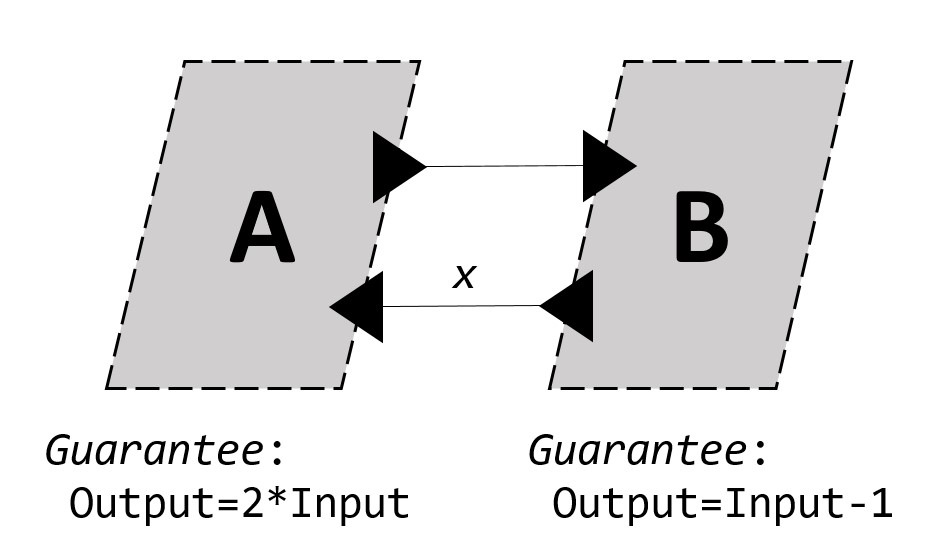
\includegraphics[width=50mm]{motivation.jpg}
\caption{An AADL Model with AGREE Contracts\label{motivationFig1}}
\end{figure}

We use the AADL model annotated with AGREE contracts in Figure \ref{motivation} to illustrate the difference between the original AGREE synchronous semantics and the AADL asynchronous semantics. The model consists of two threads A and B. The AGREE contracts associated with each thread define the input output data relationship. In the AGREE synchronous semantics, the communication between the two threads are instantaneous. And the two contracts have to be satisfied simultaneously. For example, the value of signal $x = (x_0, x_1, ...)$ is defined by the solution to the fix-point equation x = F(x), where F(x) = 2x -1. That is, $x_0 = F(x_0), x_1 = F(x_1), x_2 = F(x_2), ...$ This results in $x = (1,1,1,…)$. However, if the two threads are implemented on a single processor, they have to executed in a sequential order, e.g. $(A,B)^*$. 
%In AADL a port of a thread represents buffered communication and reading is non-blocking. If the buffer asscoated with a port is empty, a pre-defined constant value or the previous value is used. 
Given the schedule $(A,B)^*$ and an initial value x = 0,  by Kleene iteration: $x_1 = F(x_0), x_2 = F(x_1), x_3 = F(x_2),...$ This results in $x = (0,-1,-3,…)$. The two traces are different. This implies that a property proved with synchronous MoC model does not necessarily hold with asynchronous MoC. 

\begin{figure}[ht!]
\centering
\includegraphics[width=80mm]{MotivationalExample1.jpg}
\caption{An AADL Model with AGREE Contracts\label{motivationFig2}}
\end{figure}

Consider an AADL model that is consisted of 4 threads $A,B,C,D$, as shown in Figure \ref{motivationFig2}. All ports are data ports. The behavior of each thread is indicated by its AGREE contract. Thread $A$ outputs the sequence of all natural numbers. Thread B and thread C simply copy its input to the output. Thread D is a subtractor, where the second (bottom) input value is substracted from the first (top) input value. Given a schedule $(ACABD)^*$, we want to prove that the primary output $x = (1,1,1,...)$. This can be achieved with the proposed modelling framework. However, it cannot be proved directly in the current AGREE framework, where the synchrnous semantics dictates $x= (0,0,0,...)$. A special construct \emph{delay} is often introduced to model execution order in a synchronous model. However, in the example, thread $B$ and $C$ essetially downsample the data stream from thread $A$. To handle this kind of schedule, it requires much more complicated modelling mechanism than \emph{delay} in a synchornous model. Note that if the schedule is $(ABCD)^*$, then $x=(0,0,0,...)$. In fact, the data stream of each port is the same as that of the corresponding port in the synchronous model.

\begin{figure}[ht!]
\centering
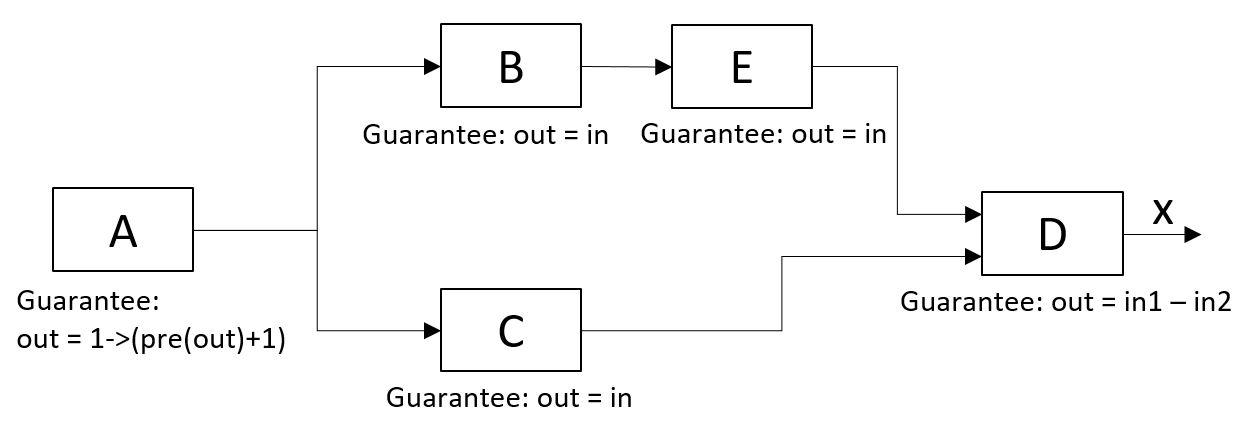
\includegraphics[width=100mm]{MotivationalExample2.jpg}
\caption{An AADL Model with AGREE Contracts\label{motivation1}}
\end{figure}
